\section{O desafio da Escassez Relativa}

A economia capitalista do século XX foi propensa ao desequilíbrio, que foi ajustada pelo remédio keynesiano, no qual foi suficiente para garantir o crescimento até o final daquele século.
No século XXI, a pauta é garantir que todos tenham acesso ao produzido, se tornou a questão central do mundo contemporâneo e com a abundância e menos perspectiva de melhora, a desigualdade fica menos tolerável.
Não obstante, a perspectiva de congelar, ou mesmo de agravar, a desigualdade da renda e da riqueza entre os países.

A Revolução da informática mantém a produtividade do capital, porém não a demanda do emprego.
Assim, contribuindo para a concentração de renda e da riqueza, por conseguinte passamos da era da escassez absoluta para a da escassez relativa.

Conclui que os desafios da escassez relativa impactam a sociedade do século XXI.
O regime democrático se demonstra a melhor alternativa para combater a desigualdade \cite{dahl2003democracy} e o Brasil comprova tal fenômeno no século XX e XXI, conforme a Figura~\ref{fig:salario-real} \cite{souza2016desigualdade}.



\begin{figure}[!ht]
    \centering
    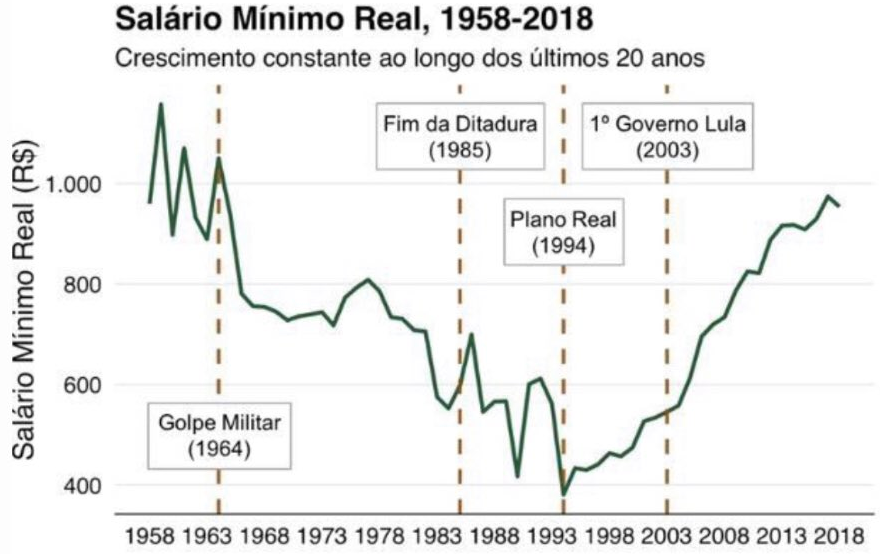
\includegraphics[width=.8\linewidth]{img/salario-minimo-real.png}
    \caption{Concentração de renda no Brasil durante 1925 à 2015. 
    Adaptado de \citeonline{barros2006desigualdade} p.231.}
    \label{fig:salario-real}
\end{figure}